The system's response to a Sum-of-Sinusoids signal with a frequency of $250 ,
Hz$ and an amplitude of $50 \mu s$ (PWM) containing $299$ frequencies within
the range of $[0.01, 30],Hz$ is employed for the identification of first-order
model parameters. The selection of the frequency range is informed by prior
endeavors aimed at capturing the system's first-order dynamics with small
signal excitations\cite{charla2022enhancing}. Table-\ref{tab::nom_in} presents
the nominal inputs along with their corresponding RPM values and validation
results. To validate the identified models, we assess their performance against
the response to a chirp signal with the same frequency range and sampling rate.

The static gain and cutoff frequencies are graphed with respect to the nominal inputs. Parameters linking them to the nominal inputs are estimated using the least-squares method.

The plot of $V_{in}$ and $K$ demonstrates the validity of their relationship when accounting for $V_{in}$ variation, expressed as:
%===
\begin{align}
    K &= V_{in} (1 + \delta v)
\end{align}
%===
\begin{figure}[h]
    \centering
    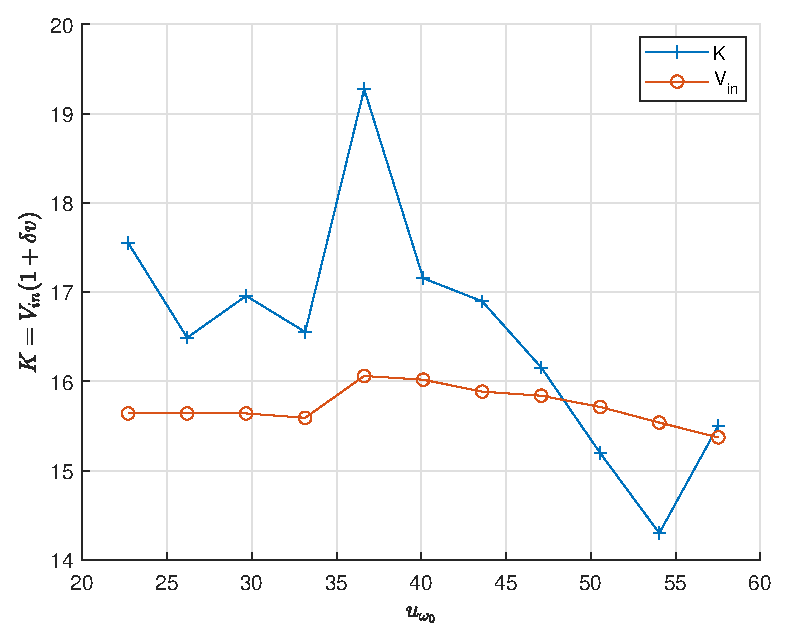
\includegraphics[width = \figsize]{./figs/small_perturbation/K-Vin.eps}
    \caption{Static gain and Voltage input}
\end{figure}
%===
\begin{figure}[h]
    \centering
    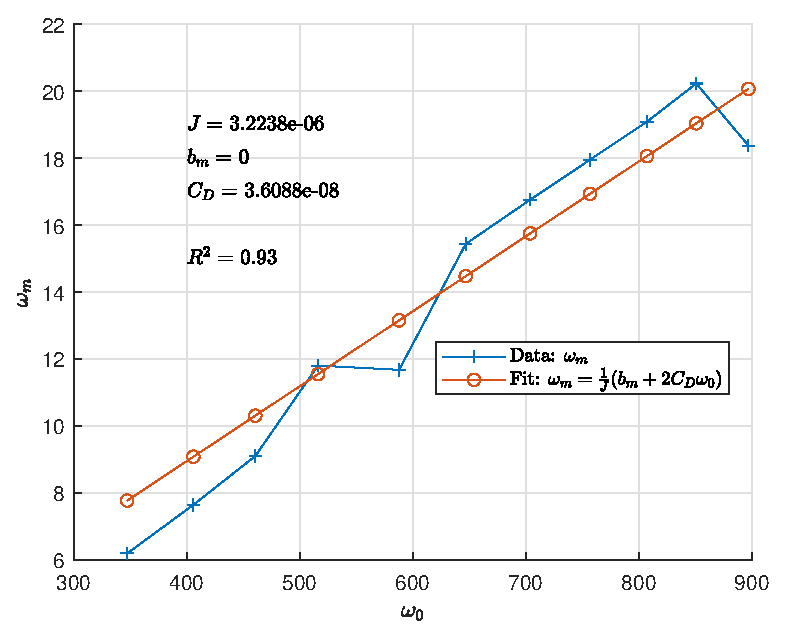
\includegraphics[width = \figsize]{./figs/small_perturbation/omega_fit.eps}
    \caption{Cut-off frequency}
\end{figure}
%===
Furthermore, based on the static gain values, we can estimate the maximum magnitude of $\abs{\delta v}$ as follows:
